
\section{\trCobordism}
\label{sec:cobordisms}

现在让我们来考虑\textbf{\trCobordism}（cobordism）。所谓\trCobordism，就是一个\trManifoldWithBoundary{} $V$，其边界 $\partial V$ 被分解为
\[
\partial V=\partial_-V\cup\partial_+V
\]
（$\partial_\pm V$ 这两部分是 $\partial V$ 中任意选定的若干\textbf{\trConnectedComponent}的并）。我们把\cref{subsec:morse-functions-adapted-fields}的构造加以推广：我们在 $V$ 内 $\partial V$ 的一个邻域上固定一个\trVectorField{} $X$（比如利用一个\trPartitionOfUnity{}来构造），它满足：
\begin{itemize}
\item 沿 $\partial_+V$ 指向外部；
\item 沿 $\partial_-V$ 指向内部。
\end{itemize}
我们在 $V$ 上构造一个\trMorseFunction{} $f$，使得
\[
df(X)<0 \qquad\text{在 } \partial V \text{ 的邻域内，}
\]
做法如下。我们先在边界的邻域内定义它，比如令
\[
\begin{cases}
f\bigl(\varphi_X^{-s}(x)\bigr)=s & \text{当 } s\in[0,\delta[\text{ 且 } x\in\partial_+V \text{ 时}\\
f\bigl(\varphi_X^{s}(x)\bigr)=-s & \text{当 } s\in[0,\delta[\text{ 且 } x\in\partial_-V \text{ 时，}
\end{cases}
\]
然后把它任意地延拓到整个 $V$ 上，最后再作一次小\trPerturbation{}，以得到一个\trMorseFunction。

于是，我们可以把 $X$ 延拓成一个\trAdapted{}于 $f$ 的\trPseudogradient{}场，并且我们仍将它记作 $X$。

让我们回忆一下（即\cref{thm:pseudogradient-transversal-boundary}）：对于这项构造，我们需要从一个\trTransverse{}于边界的\trVectorField{}出发，而且这个\trMorseFunction{}并非完全任意。

\begin{example}\label{thm:cobordism-disk-example}
在\cref{fig:hemisphere-fields}中，这个\trManifold{}是一个\trDisk{} $D^n$，而它的边界是一个\trSphere{} $S^{n-1}$。\trMorseFunction{}就是\trHeightFunction，\trVectorField{}则如图所示。在左侧，$S^{n-1}=\partial_+V$；在右侧，$S^{n-1}=\partial_-V$。
\end{example}

\begin{figure}[htbp]
\centering
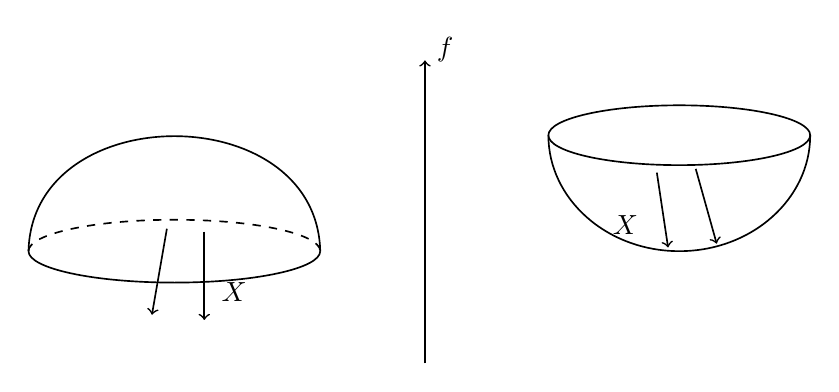
\begin{tikzpicture}[line width=0.6pt,scale=0.95]
  \draw (-1.95,0) .. controls (-1.9,2.05) and (1.9,2.05) .. (1.95,0);
  \draw (-1.95,0) arc[start angle=180,end angle=360,x radius=1.95,y radius=0.42];
  \draw[dashed] (-1.95,0) arc[start angle=180,end angle=0,x radius=1.95,y radius=0.42];
  \draw[->] (-0.1,0.3) -- (-0.3,-0.85);
  \draw[->] (0.4,0.26) -- (0.4,-0.92);
  \node at (0.8,-0.55) {$X$};
  \draw[->] (3.35,-1.5) -- (3.35,2.55);
  \node at (3.62,2.7) {$f$};
  \begin{scope}[shift={(6.75,1.55)}]
    \draw (0,0) ellipse[x radius=1.75,y radius=0.4];
    \draw (-1.75,0) arc[start angle=180,end angle=360,x radius=1.75,y radius=1.55];
    \draw[->] (-0.3,-0.5) -- (-0.15,-1.5);
    \draw[->] (0.22,-0.45) -- (0.5,-1.45);
    \node at (-0.72,-1.2) {$X$};
  \end{scope}
\end{tikzpicture}
\caption{}
\label{fig:hemisphere-fields}
\end{figure}

\begin{remark}\label{thm:cobordism-smale-modification}
我们为赋予\trPseudogradient{}场以\trSmale{}性质而作的那些修改，都是在诸\trCriticalPoint{}的邻域内进行的（因此在眼下的情形里，也就远离边界）。所以，我们可以在这里以同样的方式进行这些修改。
\end{remark}

于是，我们也可以像在无边界的情形中那样定义 $\bigl(C_{\star}(f),\partial_X\bigr)$。

\trCompact{}性的证明与关系式 $\partial_X\circ\partial_X=0$ 的证明，都同我们在无边界的情形中所给出的证明完全一样，因为诸\trCriticalPoint{}之间的所有连接都将远离边界。

\begin{remark}\label{thm:cobordism-field-boundary}
这个\trComplex{}不依赖于 $X|_{\partial V}$，只要后者保持\trTransverse{}于边界、沿 $\partial_+V$ 指向外部并沿 $\partial_-V$ 指向内部（我们可以在远离诸\trCriticalPoint{}处修改 $X$）。
\end{remark}

\begin{figure}[htbp]
\centering
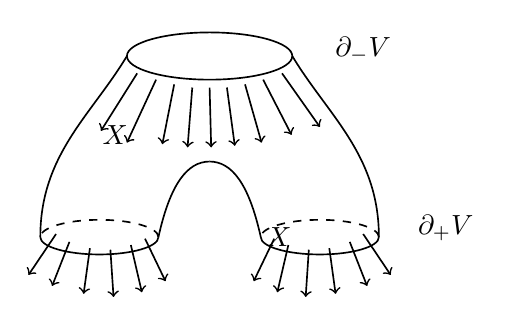
\begin{tikzpicture}[line width=0.6pt]
  \draw (-1.05,0) .. controls (-1.5,-0.75) and (-2.15,-1.25) .. (-2.15,-2.3);
  \draw (1.05,0) .. controls (1.5,-0.75) and (2.15,-1.25) .. (2.15,-2.3);
  \draw (-0.65,-2.3) .. controls (-0.5,-1.62) and (-0.28,-1.34) .. (0,-1.34);
  \draw (0,-1.34) .. controls (0.28,-1.34) and (0.5,-1.62) .. (0.65,-2.3);
  \draw (0,0) ellipse[x radius=1.05,y radius=0.3];
  \node at (1.95,0.08) {$\partial_-V$};
  \draw (-2.15,-2.3) arc[start angle=180,end angle=360,x radius=0.75,y radius=0.22];
  \draw[dashed] (-0.65,-2.3) arc[start angle=0,end angle=180,x radius=0.75,y radius=0.22];
  \draw (0.65,-2.3) arc[start angle=180,end angle=360,x radius=0.75,y radius=0.22];
  \draw[dashed] (2.15,-2.3) arc[start angle=0,end angle=180,x radius=0.75,y radius=0.22];
  \node at (3.0,-2.18) {$\partial_+V$};
  \draw[->] (-0.92,-0.22) -- (-1.38,-0.95);
  \draw[->] (-0.68,-0.3) -- (-1.05,-1.1);
  \draw[->] (-0.45,-0.36) -- (-0.6,-1.12);
  \draw[->] (-0.22,-0.4) -- (-0.28,-1.16);
  \draw[->] (0.0,-0.4) -- (0.02,-1.16);
  \draw[->] (0.22,-0.4) -- (0.32,-1.14);
  \draw[->] (0.45,-0.36) -- (0.66,-1.1);
  \draw[->] (0.68,-0.3) -- (1.04,-1.0);
  \draw[->] (0.92,-0.22) -- (1.4,-0.9);
  \node at (-1.2,-1.0) {$X$};
  \draw[->] (-1.95,-2.26) -- (-2.3,-2.78);
  \draw[->] (-1.78,-2.36) -- (-2.0,-2.92);
  \draw[->] (-1.52,-2.44) -- (-1.6,-3.02);
  \draw[->] (-1.26,-2.46) -- (-1.22,-3.06);
  \draw[->] (-1.0,-2.4) -- (-0.86,-3.0);
  \draw[->] (-0.82,-2.32) -- (-0.56,-2.86);
  \draw[->] (1.95,-2.26) -- (2.3,-2.78);
  \draw[->] (1.78,-2.36) -- (2.0,-2.92);
  \draw[->] (1.52,-2.44) -- (1.6,-3.02);
  \draw[->] (1.26,-2.46) -- (1.22,-3.06);
  \draw[->] (1.0,-2.4) -- (0.86,-3.0);
  \draw[->] (0.82,-2.32) -- (0.56,-2.86);
  \node at (0.88,-2.3) {$X$};
\end{tikzpicture}
\caption{}
\label{fig:pants-cobordism}
\end{figure}

现在让我们来证明：这个\trComplex{}的\trHomology{}既不依赖于函数，也不依赖于\trVectorField。设 $f_0$ 与 $f_1$ 是 $V$ 上的两个\trMorseFunction，各自都配有一个具有\trSmale{}性质的\trAdapted{}\trPseudogradient。我们假定这两个\trVectorField{} $X_0$ 与 $X_1$ 在边界的邻域内相重合。让我们像前面那样选取一条从 $f_0$ 到 $f_1$ 的路径 $f_t$，并假定它在两个端点附近是\trStationary{}的：
\[
f_t=f_0 \quad\text{对 } t\le\tfrac{1}{3}
\qquad\text{且}\qquad
f_t=f_1 \quad\text{对 } t\ge\tfrac{2}{3}\text{。}
\]
我们还假定在 $\partial V$ 的邻域内 $df_t(X)<0$。我们把 $f_t$ 延拓成 $[-1/3,0]$ 与 $[1,4/3]$ 上的\trStationary{}函数。我们像前面那样使用一个函数 $g$（\cref{fig:function-g}），使得
\[
\forall t\in\bigl[\tfrac{1}{3},\tfrac{2}{3}\bigr],\ \forall x\in V,\qquad
g'(t)+\frac{\partial f_t(x)}{\partial t}<0\text{。}
\]
如同在独立性的证明中那样，我们令\footnote{译注：原书此式印作 $g(x)$；$g$ 即\cref{fig:function-g}中的那个单元函数，上式用的是 $g'(t)$，下文的 $\operatorname{grad}g$ 也只作用于变量 $t$，故应为 $g(t)$；此处径改。——译者注}
\[
F(x,t)=f_t(x)+g(t)\qquad\text{对 } (x,t)\in V\times\bigl[-\tfrac{1}{3},\tfrac{4}{3}\bigr]\text{。}
\]
再一次如同在那个证明中那样，$F$ 的诸\trCriticalPoint{}就是\trSection{} $t=0$ 中 $f_0$ 的那些与\trSection{} $t=1$ 中 $f_1$ 的那些，其中位于\trSection{} $t=0$ 中的那些有一个\trIndex{}跳跃。

最后，我们为 $F$ 构造一个\trPseudogradient{} $\widetilde{X}$，使得
\[
\widetilde{X}=
\begin{cases}
X-\operatorname{grad}g & \text{在 } \partial V\times[0,1] \text{ 附近}\\
X_0-\operatorname{grad}g & \text{在 } V\times\bigl[-\tfrac{1}{3},\tfrac{1}{3}\bigr] \text{ 上}\\
X_1-\operatorname{grad}g & \text{在 } V\times\bigl[\tfrac{2}{3},\tfrac{4}{3}\bigr] \text{ 上。}
\end{cases}
\]
于是我们只需再取一个小\trPerturbation{}，便可获得\trSmale{}性质。简言之，我们构成\trComplex{} $\bigl(C_{\star}(F),\partial_{\widetilde{X}}\bigr)$。如同在无边界的情形中那样，我们有
\[
\bigl(C_k(F),\partial_{\widetilde{X}}\bigr)
=\Bigl(C_{k-1}(f_0)\oplus C_k(f_1),
\begin{pmatrix}\partial_{X_0} & 0\\ \Phi_{\widetilde{X}} & \partial_{X_1}\end{pmatrix}\Bigr)\text{，}
\]
它定义了\trComplex{}的一个\trMorphism
\[
\Phi_{\widetilde{X}}\colon\bigl(C_{\star}(f_0),\partial_{X_0}\bigr)
\longrightarrow\bigl(C_{\star}(f_1),\partial_{X_1}\bigr)\text{，}
\]
我们可以像前面那样证明：它在\trHomology{}中诱导出一个\trIsomorphism。

归结起来：在这一情形中，\trComplex{}的\trHomology{}只依赖于 $V$ 以及 $\partial V=\partial_+V\cup\partial_-V$ 这一边界分解。

还请注意，$\Phi^F_{\star}$ 不依赖于 $F$。为使你自己确信这一点，对于一个别的“\trInterpolation” $F'$，只需在\cref{thm:chain-morphism-isomorphism}的证明的第三步中取 $G=\operatorname{Id}$ 与 $H=F'$ 便可。
